\documentclass[]{article}
\usepackage{lmodern}
\usepackage{amssymb,amsmath}
\usepackage{ifxetex,ifluatex}
\usepackage{fixltx2e} % provides \textsubscript
\ifnum 0\ifxetex 1\fi\ifluatex 1\fi=0 % if pdftex
  \usepackage[T1]{fontenc}
  \usepackage[utf8]{inputenc}
\else % if luatex or xelatex
  \ifxetex
    \usepackage{mathspec}
  \else
    \usepackage{fontspec}
  \fi
  \defaultfontfeatures{Ligatures=TeX,Scale=MatchLowercase}
\fi
% use upquote if available, for straight quotes in verbatim environments
\IfFileExists{upquote.sty}{\usepackage{upquote}}{}
% use microtype if available
\IfFileExists{microtype.sty}{%
\usepackage{microtype}
\UseMicrotypeSet[protrusion]{basicmath} % disable protrusion for tt fonts
}{}
\usepackage[margin=1in]{geometry}
\usepackage{hyperref}
\hypersetup{unicode=true,
            pdfborder={0 0 0},
            breaklinks=true}
\urlstyle{same}  % don't use monospace font for urls
\usepackage{color}
\usepackage{fancyvrb}
\newcommand{\VerbBar}{|}
\newcommand{\VERB}{\Verb[commandchars=\\\{\}]}
\DefineVerbatimEnvironment{Highlighting}{Verbatim}{commandchars=\\\{\}}
% Add ',fontsize=\small' for more characters per line
\usepackage{framed}
\definecolor{shadecolor}{RGB}{248,248,248}
\newenvironment{Shaded}{\begin{snugshade}}{\end{snugshade}}
\newcommand{\KeywordTok}[1]{\textcolor[rgb]{0.13,0.29,0.53}{\textbf{#1}}}
\newcommand{\DataTypeTok}[1]{\textcolor[rgb]{0.13,0.29,0.53}{#1}}
\newcommand{\DecValTok}[1]{\textcolor[rgb]{0.00,0.00,0.81}{#1}}
\newcommand{\BaseNTok}[1]{\textcolor[rgb]{0.00,0.00,0.81}{#1}}
\newcommand{\FloatTok}[1]{\textcolor[rgb]{0.00,0.00,0.81}{#1}}
\newcommand{\ConstantTok}[1]{\textcolor[rgb]{0.00,0.00,0.00}{#1}}
\newcommand{\CharTok}[1]{\textcolor[rgb]{0.31,0.60,0.02}{#1}}
\newcommand{\SpecialCharTok}[1]{\textcolor[rgb]{0.00,0.00,0.00}{#1}}
\newcommand{\StringTok}[1]{\textcolor[rgb]{0.31,0.60,0.02}{#1}}
\newcommand{\VerbatimStringTok}[1]{\textcolor[rgb]{0.31,0.60,0.02}{#1}}
\newcommand{\SpecialStringTok}[1]{\textcolor[rgb]{0.31,0.60,0.02}{#1}}
\newcommand{\ImportTok}[1]{#1}
\newcommand{\CommentTok}[1]{\textcolor[rgb]{0.56,0.35,0.01}{\textit{#1}}}
\newcommand{\DocumentationTok}[1]{\textcolor[rgb]{0.56,0.35,0.01}{\textbf{\textit{#1}}}}
\newcommand{\AnnotationTok}[1]{\textcolor[rgb]{0.56,0.35,0.01}{\textbf{\textit{#1}}}}
\newcommand{\CommentVarTok}[1]{\textcolor[rgb]{0.56,0.35,0.01}{\textbf{\textit{#1}}}}
\newcommand{\OtherTok}[1]{\textcolor[rgb]{0.56,0.35,0.01}{#1}}
\newcommand{\FunctionTok}[1]{\textcolor[rgb]{0.00,0.00,0.00}{#1}}
\newcommand{\VariableTok}[1]{\textcolor[rgb]{0.00,0.00,0.00}{#1}}
\newcommand{\ControlFlowTok}[1]{\textcolor[rgb]{0.13,0.29,0.53}{\textbf{#1}}}
\newcommand{\OperatorTok}[1]{\textcolor[rgb]{0.81,0.36,0.00}{\textbf{#1}}}
\newcommand{\BuiltInTok}[1]{#1}
\newcommand{\ExtensionTok}[1]{#1}
\newcommand{\PreprocessorTok}[1]{\textcolor[rgb]{0.56,0.35,0.01}{\textit{#1}}}
\newcommand{\AttributeTok}[1]{\textcolor[rgb]{0.77,0.63,0.00}{#1}}
\newcommand{\RegionMarkerTok}[1]{#1}
\newcommand{\InformationTok}[1]{\textcolor[rgb]{0.56,0.35,0.01}{\textbf{\textit{#1}}}}
\newcommand{\WarningTok}[1]{\textcolor[rgb]{0.56,0.35,0.01}{\textbf{\textit{#1}}}}
\newcommand{\AlertTok}[1]{\textcolor[rgb]{0.94,0.16,0.16}{#1}}
\newcommand{\ErrorTok}[1]{\textcolor[rgb]{0.64,0.00,0.00}{\textbf{#1}}}
\newcommand{\NormalTok}[1]{#1}
\usepackage{graphicx,grffile}
\makeatletter
\def\maxwidth{\ifdim\Gin@nat@width>\linewidth\linewidth\else\Gin@nat@width\fi}
\def\maxheight{\ifdim\Gin@nat@height>\textheight\textheight\else\Gin@nat@height\fi}
\makeatother
% Scale images if necessary, so that they will not overflow the page
% margins by default, and it is still possible to overwrite the defaults
% using explicit options in \includegraphics[width, height, ...]{}
\setkeys{Gin}{width=\maxwidth,height=\maxheight,keepaspectratio}
\IfFileExists{parskip.sty}{%
\usepackage{parskip}
}{% else
\setlength{\parindent}{0pt}
\setlength{\parskip}{6pt plus 2pt minus 1pt}
}
\setlength{\emergencystretch}{3em}  % prevent overfull lines
\providecommand{\tightlist}{%
  \setlength{\itemsep}{0pt}\setlength{\parskip}{0pt}}
\setcounter{secnumdepth}{0}
% Redefines (sub)paragraphs to behave more like sections
\ifx\paragraph\undefined\else
\let\oldparagraph\paragraph
\renewcommand{\paragraph}[1]{\oldparagraph{#1}\mbox{}}
\fi
\ifx\subparagraph\undefined\else
\let\oldsubparagraph\subparagraph
\renewcommand{\subparagraph}[1]{\oldsubparagraph{#1}\mbox{}}
\fi

%%% Use protect on footnotes to avoid problems with footnotes in titles
\let\rmarkdownfootnote\footnote%
\def\footnote{\protect\rmarkdownfootnote}

%%% Change title format to be more compact
\usepackage{titling}

% Create subtitle command for use in maketitle
\newcommand{\subtitle}[1]{
  \posttitle{
    \begin{center}\large#1\end{center}
    }
}

\setlength{\droptitle}{-2em}

  \title{}
    \pretitle{\vspace{\droptitle}}
  \posttitle{}
    \author{}
    \preauthor{}\postauthor{}
    \date{}
    \predate{}\postdate{}
  

\begin{document}

\begin{center}\rule{0.5\linewidth}{\linethickness}\end{center}

title: ``Chen lab RNA-seq'' output: html\_notebook \#human cell lines \#
si RNA knockdown experiment

\begin{Shaded}
\begin{Highlighting}[]
\KeywordTok{library}\NormalTok{(pheatmap)}
\KeywordTok{library}\NormalTok{(edgeR)}
\end{Highlighting}
\end{Shaded}

\begin{verbatim}
## Loading required package: limma
\end{verbatim}

\begin{Shaded}
\begin{Highlighting}[]
\KeywordTok{library}\NormalTok{(DESeq2)}
\end{Highlighting}
\end{Shaded}

\begin{verbatim}
## Loading required package: S4Vectors
\end{verbatim}

\begin{verbatim}
## Loading required package: stats4
\end{verbatim}

\begin{verbatim}
## Loading required package: BiocGenerics
\end{verbatim}

\begin{verbatim}
## Loading required package: parallel
\end{verbatim}

\begin{verbatim}
## 
## Attaching package: 'BiocGenerics'
\end{verbatim}

\begin{verbatim}
## The following objects are masked from 'package:parallel':
## 
##     clusterApply, clusterApplyLB, clusterCall, clusterEvalQ,
##     clusterExport, clusterMap, parApply, parCapply, parLapply,
##     parLapplyLB, parRapply, parSapply, parSapplyLB
\end{verbatim}

\begin{verbatim}
## The following object is masked from 'package:limma':
## 
##     plotMA
\end{verbatim}

\begin{verbatim}
## The following objects are masked from 'package:stats':
## 
##     IQR, mad, sd, var, xtabs
\end{verbatim}

\begin{verbatim}
## The following objects are masked from 'package:base':
## 
##     anyDuplicated, append, as.data.frame, basename, cbind,
##     colMeans, colnames, colSums, dirname, do.call, duplicated,
##     eval, evalq, Filter, Find, get, grep, grepl, intersect,
##     is.unsorted, lapply, lengths, Map, mapply, match, mget, order,
##     paste, pmax, pmax.int, pmin, pmin.int, Position, rank, rbind,
##     Reduce, rowMeans, rownames, rowSums, sapply, setdiff, sort,
##     table, tapply, union, unique, unsplit, which, which.max,
##     which.min
\end{verbatim}

\begin{verbatim}
## 
## Attaching package: 'S4Vectors'
\end{verbatim}

\begin{verbatim}
## The following object is masked from 'package:base':
## 
##     expand.grid
\end{verbatim}

\begin{verbatim}
## Loading required package: IRanges
\end{verbatim}

\begin{verbatim}
## Loading required package: GenomicRanges
\end{verbatim}

\begin{verbatim}
## Loading required package: GenomeInfoDb
\end{verbatim}

\begin{verbatim}
## Loading required package: SummarizedExperiment
\end{verbatim}

\begin{verbatim}
## Loading required package: Biobase
\end{verbatim}

\begin{verbatim}
## Welcome to Bioconductor
## 
##     Vignettes contain introductory material; view with
##     'browseVignettes()'. To cite Bioconductor, see
##     'citation("Biobase")', and for packages 'citation("pkgname")'.
\end{verbatim}

\begin{verbatim}
## Loading required package: DelayedArray
\end{verbatim}

\begin{verbatim}
## Loading required package: matrixStats
\end{verbatim}

\begin{verbatim}
## 
## Attaching package: 'matrixStats'
\end{verbatim}

\begin{verbatim}
## The following objects are masked from 'package:Biobase':
## 
##     anyMissing, rowMedians
\end{verbatim}

\begin{verbatim}
## Loading required package: BiocParallel
\end{verbatim}

\begin{verbatim}
## 
## Attaching package: 'DelayedArray'
\end{verbatim}

\begin{verbatim}
## The following objects are masked from 'package:matrixStats':
## 
##     colMaxs, colMins, colRanges, rowMaxs, rowMins, rowRanges
\end{verbatim}

\begin{verbatim}
## The following objects are masked from 'package:base':
## 
##     aperm, apply
\end{verbatim}

Read in files

\begin{Shaded}
\begin{Highlighting}[]
\NormalTok{filename =}\StringTok{ "~/Downloads/readcounts.txt"}
\NormalTok{counts1 =}\StringTok{ }\KeywordTok{read.table}\NormalTok{(filename, }\DataTypeTok{header =}\NormalTok{ T, }\DataTypeTok{stringsAsFactors =}\NormalTok{ F) }
\KeywordTok{rownames}\NormalTok{(counts1) =}\StringTok{ }\NormalTok{counts1}\OperatorTok{$}\NormalTok{Geneid}
\end{Highlighting}
\end{Shaded}

Remove metadata (Gene, coordinates, etc)

\begin{Shaded}
\begin{Highlighting}[]
\NormalTok{counts2 =}\StringTok{ }\NormalTok{counts1[,}\DecValTok{7}\OperatorTok{:}\KeywordTok{ncol}\NormalTok{(counts1)]}
\KeywordTok{colnames}\NormalTok{(counts2) =}\StringTok{ }\KeywordTok{sub}\NormalTok{(}\StringTok{"_1_algn_Aligned"}\NormalTok{, }\StringTok{""}\NormalTok{, }\KeywordTok{matrix}\NormalTok{(}\KeywordTok{unlist}\NormalTok{(}\KeywordTok{strsplit}\NormalTok{(}\KeywordTok{colnames}\NormalTok{(counts2), }\StringTok{"}\CharTok{\textbackslash{}\textbackslash{}}\StringTok{."}\NormalTok{)), }\DataTypeTok{byrow =}\NormalTok{T, }\DataTypeTok{ncol=}\DecValTok{6}\NormalTok{)[,}\DecValTok{3}\NormalTok{])}
\end{Highlighting}
\end{Shaded}

Filter out genes with low and high counts ( high counts might be
mitochondrial genes)

\begin{Shaded}
\begin{Highlighting}[]
\NormalTok{keep =}\StringTok{ }\KeywordTok{rowMeans}\NormalTok{(counts2) }\OperatorTok{>}\StringTok{ }\DecValTok{5} \OperatorTok{&}\StringTok{ }\KeywordTok{rowMeans}\NormalTok{(counts2) }\OperatorTok{<}\StringTok{ }\DecValTok{5000} 
\NormalTok{counts3 =}\StringTok{ }\NormalTok{counts2[keep,]}
\end{Highlighting}
\end{Shaded}

Add count of 1 so that I can take the log later

\begin{Shaded}
\begin{Highlighting}[]
\NormalTok{counts4 =}\StringTok{ }\NormalTok{counts3 }\OperatorTok{+}\StringTok{ }\DecValTok{1}
\end{Highlighting}
\end{Shaded}

Take the log (RPKM)

\begin{Shaded}
\begin{Highlighting}[]
\NormalTok{y <-}\StringTok{ }\KeywordTok{DGEList}\NormalTok{(}\DataTypeTok{counts=}\NormalTok{counts4)}
\NormalTok{fpkm_log_matrix =}\StringTok{ }\KeywordTok{rpkm}\NormalTok{ (y, }\DataTypeTok{gene.length=}\NormalTok{counts1[keep,}\StringTok{"Length"}\NormalTok{], }\DataTypeTok{log =} \OtherTok{TRUE}\NormalTok{)}
\end{Highlighting}
\end{Shaded}

scatterplot pairwise

Dendrogram

\begin{Shaded}
\begin{Highlighting}[]
\CommentTok{# }
\CommentTok{#par(cex=1,font=3)}
\NormalTok{hc2 <-}\StringTok{ }\KeywordTok{hclust}\NormalTok{(stats}\OperatorTok{::}\KeywordTok{dist}\NormalTok{(}\KeywordTok{t}\NormalTok{(fpkm_log_matrix), }\DataTypeTok{method=}\StringTok{"minkowski"}\NormalTok{), }\StringTok{"ward.D2"}\NormalTok{)}
\CommentTok{#par(mar=c(10, 4, 4, 10), pty='s')}
\KeywordTok{plot}\NormalTok{(hc2, }\DataTypeTok{lwd=}\DecValTok{4}\NormalTok{, }\DataTypeTok{lty=}\DecValTok{1}\NormalTok{, }\DataTypeTok{col=}\StringTok{"black"}\NormalTok{, }\DataTypeTok{col.lab=}\StringTok{"red"}\NormalTok{, }\DataTypeTok{xlab=}\StringTok{"Samples"}\NormalTok{, }\DataTypeTok{main=}\StringTok{"Samples clustered by log2(FPKM+1) using Ward's clustering & Euclidean distance"}\NormalTok{)}
\end{Highlighting}
\end{Shaded}

\includegraphics{plots_and_edgeR_analysis_files/figure-latex/unnamed-chunk-8-1.pdf}
Some replicates don't cluster. Samples cluster by cell type.

Setup up design matrix for PCA plot

\begin{Shaded}
\begin{Highlighting}[]
\NormalTok{groupNamesPerSample =}\StringTok{ }\KeywordTok{matrix}\NormalTok{ (}\KeywordTok{unlist}\NormalTok{(}\KeywordTok{strsplit}\NormalTok{(}\KeywordTok{colnames}\NormalTok{(counts4), }\StringTok{"_"}\NormalTok{)), }\DataTypeTok{byrow=}\NormalTok{T, }\DataTypeTok{ncol=}\DecValTok{4}\NormalTok{) [,}\DecValTok{1}\NormalTok{]}
\NormalTok{groupNamesPerSample =}\StringTok{ }\KeywordTok{unlist}\NormalTok{( }\KeywordTok{lapply}\NormalTok{ (groupNamesPerSample, }\ControlFlowTok{function}\NormalTok{(x) }\KeywordTok{sub}\NormalTok{(}\StringTok{"S475"}\NormalTok{, }\StringTok{""}\NormalTok{, }\KeywordTok{sub}\NormalTok{(}\StringTok{"S449"}\NormalTok{, }\StringTok{""}\NormalTok{, }\KeywordTok{sub}\NormalTok{(}\StringTok{"PLC"}\NormalTok{, }\StringTok{""}\NormalTok{, }\KeywordTok{sub}\NormalTok{(}\StringTok{"Focus"}\NormalTok{, }\StringTok{""}\NormalTok{, x))))) )}
\NormalTok{conditionFactor  <-}\StringTok{ }\KeywordTok{factor}\NormalTok{(groupNamesPerSample)}
\NormalTok{subjectgroup =}\StringTok{ }\KeywordTok{matrix}\NormalTok{ (}\KeywordTok{unlist}\NormalTok{(}\KeywordTok{strsplit}\NormalTok{(}\KeywordTok{colnames}\NormalTok{(counts4), }\StringTok{"_"}\NormalTok{)), }\DataTypeTok{byrow=}\NormalTok{T, }\DataTypeTok{ncol=}\DecValTok{4}\NormalTok{) [,}\DecValTok{1}\NormalTok{]}
\NormalTok{subjectgroup =}\StringTok{ }\KeywordTok{unlist}\NormalTok{( }\KeywordTok{lapply}\NormalTok{ (subjectgroup, }\ControlFlowTok{function}\NormalTok{(x) }\KeywordTok{sub}\NormalTok{(}\StringTok{"SC"}\NormalTok{, }\StringTok{""}\NormalTok{, }\KeywordTok{sub}\NormalTok{(}\StringTok{"YT"}\NormalTok{, }\StringTok{""}\NormalTok{, }\KeywordTok{sub}\NormalTok{(}\StringTok{"T"}\NormalTok{, }\StringTok{""}\NormalTok{, }\KeywordTok{sub}\NormalTok{(}\StringTok{"Y"}\NormalTok{, }\StringTok{""}\NormalTok{, x))))) )}
\NormalTok{Subject <-}\StringTok{ }\KeywordTok{factor}\NormalTok{(subjectgroup)}
\end{Highlighting}
\end{Shaded}

PCA plot

\begin{Shaded}
\begin{Highlighting}[]
\KeywordTok{library}\NormalTok{(ggplot2)}
\NormalTok{cold <-}\StringTok{ }\KeywordTok{data.frame}\NormalTok{(}\StringTok{"conditionFactor"}\NormalTok{=conditionFactor, }\StringTok{"Subject"}\NormalTok{=Subject) }\CommentTok{#"sample_name"=colnames(counts4)}
\NormalTok{design_matrix <-}\StringTok{ }\KeywordTok{model.matrix}\NormalTok{( }\OperatorTok{~}\NormalTok{Subject }\OperatorTok{+}\StringTok{ }\NormalTok{conditionFactor)}
\NormalTok{ddsMat <-}\StringTok{ }\NormalTok{DESeq2}\OperatorTok{::}\KeywordTok{DESeqDataSetFromMatrix}\NormalTok{(}\DataTypeTok{countData=}\NormalTok{counts4, }\DataTypeTok{colData=}\NormalTok{cold, }\DataTypeTok{design=}\OperatorTok{~}\NormalTok{conditionFactor);}
\end{Highlighting}
\end{Shaded}

\begin{verbatim}
## converting counts to integer mode
\end{verbatim}

\begin{Shaded}
\begin{Highlighting}[]
\KeywordTok{colnames}\NormalTok{(ddsMat) <-}\StringTok{ }\KeywordTok{colnames}\NormalTok{(counts4)}
\NormalTok{rld <-}\StringTok{ }\NormalTok{DESeq2}\OperatorTok{::}\KeywordTok{rlog}\NormalTok{(ddsMat) }\CommentTok{# LOG TRANSFORMED.}
\CommentTok{#rld <- DESeq2::rlog(ddsMat, blind=blind_status) }

\NormalTok{pca              <-}\StringTok{ }\KeywordTok{prcomp}\NormalTok{(}\KeywordTok{t}\NormalTok{(}\KeywordTok{assay}\NormalTok{(rld)))}
\NormalTok{allPer.vec       <-}\StringTok{ }\DecValTok{100} \OperatorTok{*}\StringTok{ }\KeywordTok{summary}\NormalTok{(pca)}\OperatorTok{$}\NormalTok{importance[}\DecValTok{2}\NormalTok{,]}
\NormalTok{allPer.text      <-}\StringTok{ }\KeywordTok{paste}\NormalTok{(}\KeywordTok{format}\NormalTok{(allPer.vec,}\DataTypeTok{digits=}\DecValTok{0}\NormalTok{, }\DataTypeTok{nsmall=}\DecValTok{1}\NormalTok{, }\DataTypeTok{scientific=}\OtherTok{FALSE}\NormalTok{), }\StringTok{"%"}\NormalTok{, }\DataTypeTok{sep=}\StringTok{''}\NormalTok{)}
\NormalTok{allPerLabels.vec <-}\StringTok{ }\KeywordTok{paste}\NormalTok{(}\KeywordTok{names}\NormalTok{(allPer.vec), }\StringTok{"}\CharTok{\textbackslash{}n}\StringTok{"}\NormalTok{, allPer.text, }\DataTypeTok{sep=}\StringTok{''}\NormalTok{)}

\KeywordTok{barplot}\NormalTok{(allPer.vec, }\DataTypeTok{main=}\StringTok{"PCA: % variance explained by each component}\CharTok{\textbackslash{}n}\StringTok{"}\NormalTok{ , }\DataTypeTok{ylim=}\KeywordTok{c}\NormalTok{(}\DecValTok{0}\NormalTok{,}\DecValTok{100}\NormalTok{), }\DataTypeTok{names.arg=}\NormalTok{allPerLabels.vec)}
\end{Highlighting}
\end{Shaded}

\includegraphics{plots_and_edgeR_analysis_files/figure-latex/unnamed-chunk-10-1.pdf}

\begin{Shaded}
\begin{Highlighting}[]
\NormalTok{d <-}\StringTok{ }\KeywordTok{data.frame}\NormalTok{(pca}\OperatorTok{$}\NormalTok{x, }\DataTypeTok{group=}\NormalTok{conditionFactor, Subject, }\DataTypeTok{name=}\KeywordTok{colnames}\NormalTok{(rld)) }\CommentTok{# returns PC1, PC2, ... PC8... etc}
\NormalTok{ppp <-}\StringTok{ }\KeywordTok{ggplot}\NormalTok{(d, }\KeywordTok{aes_string}\NormalTok{(}\DataTypeTok{x=}\StringTok{"PC1"}\NormalTok{, }\DataTypeTok{y=}\StringTok{"PC2"}\NormalTok{, }\DataTypeTok{shape=}\StringTok{"Subject"}\NormalTok{, }\DataTypeTok{color=}\StringTok{"group"}\NormalTok{))}
\NormalTok{ppp <-}\StringTok{ }\NormalTok{ppp }\OperatorTok{+}\StringTok{ }\KeywordTok{geom_point}\NormalTok{(}\DataTypeTok{size=}\DecValTok{6}\NormalTok{)}
\KeywordTok{plot}\NormalTok{(ppp)}
\end{Highlighting}
\end{Shaded}

\includegraphics{plots_and_edgeR_analysis_files/figure-latex/unnamed-chunk-10-2.pdf}
Samples seem to cluster by cell type. S449 and S475 appear to be very
similar. Replicates cluster together mostly.

Concatenate samples with replicates

\begin{Shaded}
\begin{Highlighting}[]
\CommentTok{#done manually using counts3 because I don't want to use matrix counts with 1 added to the value}
\NormalTok{counts5 =}\StringTok{ }\KeywordTok{data.frame}\NormalTok{(}
\NormalTok{            counts3}\OperatorTok{$}\NormalTok{FocusSC_USR17001380L_HJHCJBBXX_L6}
\NormalTok{          , counts3}\OperatorTok{$}\NormalTok{FocusT_USR17001382L_HJHCJBBXX_L7 }\OperatorTok{+}\StringTok{ }\NormalTok{counts3}\OperatorTok{$}\NormalTok{FocusT_USR17001382L_HKF5JBBXX_L1}
\NormalTok{          , counts3}\OperatorTok{$}\NormalTok{FocusYT_USR17001383L_hkff7BBXX_L1 }\OperatorTok{+}\StringTok{ }\NormalTok{counts3}\OperatorTok{$}\NormalTok{FocusYT_USR17001383L_HKY5KBBXX_L1}
\NormalTok{          , counts3}\OperatorTok{$}\NormalTok{FocusY_USR17001381L_HJHCJBBXX_L6}
          
\NormalTok{          , counts3}\OperatorTok{$}\NormalTok{PLCSC_USR17002043L_HJHCJBBXX_L7}
\NormalTok{          , counts3}\OperatorTok{$}\NormalTok{PLCT_USR17002044L_HJHCJBBXX_L7}
\NormalTok{          , counts3}\OperatorTok{$}\NormalTok{PLCYT_USR17001379L_HJHCJBBXX_L6}
\NormalTok{          , counts3}\OperatorTok{$}\NormalTok{PLCY_USR17001377L_HJHCJBBXX_L6}
          
\NormalTok{          , counts3}\OperatorTok{$}\NormalTok{S449SC_USR17001384L_HJHCJBBXX_L7}
\NormalTok{          , counts3}\OperatorTok{$}\NormalTok{S449T_USR17001386L_HJHCJBBXX_L7 }
\NormalTok{          , counts3}\OperatorTok{$}\NormalTok{S449YT_USR17002046L_HJHCJBBXX_L7 }\OperatorTok{+}\StringTok{ }\NormalTok{counts3}\OperatorTok{$}\NormalTok{S449YT_USR17002046L_HKF5JBBXX_L3 }
\NormalTok{          , counts3}\OperatorTok{$}\NormalTok{S449Y_USR17001385L_HJHCJBBXX_L7 }\OperatorTok{+}\StringTok{ }\NormalTok{counts3}\OperatorTok{$}\NormalTok{S449Y_USR17001385L_HKF5JBBXX_L3}
          
\NormalTok{          , counts3}\OperatorTok{$}\NormalTok{S475SC_USR17001372L_HJHCJBBXX_L6}
\NormalTok{          , counts3}\OperatorTok{$}\NormalTok{S475T_USR17001374L_HJHCJBBXX_L6}
\NormalTok{          , counts3}\OperatorTok{$}\NormalTok{S475YT_USR17001375L_HJHCJBBXX_L6}
\NormalTok{          , counts3}\OperatorTok{$}\NormalTok{S475Y_USR17001373L_HJHCJBBXX_L6 }
\NormalTok{          )}

\KeywordTok{colnames}\NormalTok{(counts5) =}\StringTok{ }\KeywordTok{unlist}\NormalTok{(}\KeywordTok{lapply}\NormalTok{ (}\KeywordTok{strsplit}\NormalTok{(}\KeywordTok{sub}\NormalTok{(}\StringTok{"counts3."}\NormalTok{, }\StringTok{""}\NormalTok{ ,}\KeywordTok{colnames}\NormalTok{(counts5)) , }\StringTok{"_"}\NormalTok{), }\StringTok{`}\DataTypeTok{[[}\StringTok{`}\NormalTok{, }\DecValTok{1}\NormalTok{))}
\end{Highlighting}
\end{Shaded}

TODO: most highly variable genes

\begin{Shaded}
\begin{Highlighting}[]
\NormalTok{HEATMAP_HEIGHT <-}\StringTok{ }\DecValTok{45} \CommentTok{# inchescol}
\NormalTok{HEATMAP_WIDTH  <-}\StringTok{ }\DecValTok{15}

\KeywordTok{pheatmap}\NormalTok{(counts5[}\DecValTok{1}\OperatorTok{:}\DecValTok{500}\NormalTok{,],}
\NormalTok{         , }\DataTypeTok{width=}\NormalTok{HEATMAP_WIDTH, }\DataTypeTok{height=}\NormalTok{HEATMAP_HEIGHT}
\NormalTok{         , }\DataTypeTok{scale=}\StringTok{"row"}  \CommentTok{# actually scale each row}
\NormalTok{         , }\DataTypeTok{clustering_distance_rows=}\StringTok{"correlation"} \CommentTok{# or: euclidean}
\NormalTok{         , }\DataTypeTok{clustering_distance_cols=}\StringTok{"correlation"}
\NormalTok{         , }\DataTypeTok{clustering_method=}\StringTok{"complete"}
\NormalTok{         , }\DataTypeTok{display_numbers=}\OtherTok{FALSE}
\NormalTok{         , }\DataTypeTok{border_color=}\StringTok{"#00000000"} \CommentTok{# note: the last two digits here are the alpha channel/ transparency}
\NormalTok{         , }\DataTypeTok{show_rownames=}\OtherTok{FALSE}\NormalTok{, }\DataTypeTok{show_colnames =} \OtherTok{FALSE}
\NormalTok{         , }\DataTypeTok{fontsize_row=}\FloatTok{3.5}\NormalTok{)}
\end{Highlighting}
\end{Shaded}

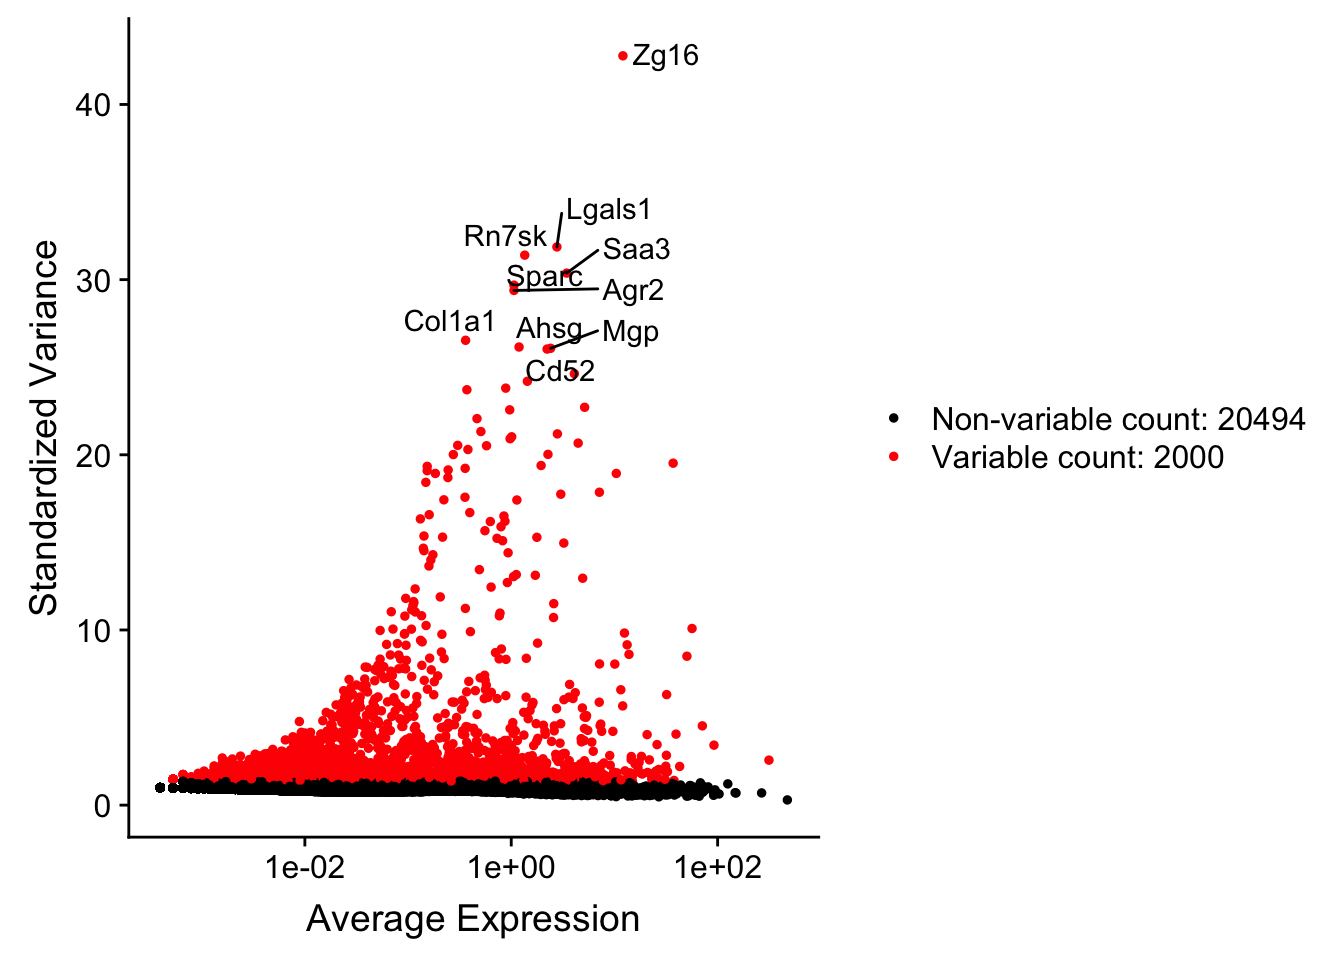
\includegraphics{plots_and_edgeR_analysis_files/figure-latex/unnamed-chunk-12-1.pdf}
Setup up design matrix for DE

\begin{Shaded}
\begin{Highlighting}[]
\NormalTok{Condition =}\StringTok{ }\KeywordTok{unlist}\NormalTok{( }\KeywordTok{lapply}\NormalTok{ (}\KeywordTok{colnames}\NormalTok{(counts5), }\ControlFlowTok{function}\NormalTok{(x) }\KeywordTok{sub}\NormalTok{(}\StringTok{"S475"}\NormalTok{, }\StringTok{""}\NormalTok{, }\KeywordTok{sub}\NormalTok{(}\StringTok{"S449"}\NormalTok{, }\StringTok{""}\NormalTok{, }\KeywordTok{sub}\NormalTok{(}\StringTok{"PLC"}\NormalTok{, }\StringTok{""}\NormalTok{, }\KeywordTok{sub}\NormalTok{(}\StringTok{"Focus"}\NormalTok{, }\StringTok{""}\NormalTok{, x))))) )}
\NormalTok{Condition  <-}\StringTok{ }\KeywordTok{factor}\NormalTok{(Condition)}
\NormalTok{Subject2 =}\StringTok{ }\KeywordTok{unlist}\NormalTok{( }\KeywordTok{lapply}\NormalTok{ (}\KeywordTok{colnames}\NormalTok{(counts5), }\ControlFlowTok{function}\NormalTok{(x) }\KeywordTok{sub}\NormalTok{(}\StringTok{"SC"}\NormalTok{, }\StringTok{""}\NormalTok{, }\KeywordTok{sub}\NormalTok{(}\StringTok{"YT"}\NormalTok{, }\StringTok{""}\NormalTok{, }\KeywordTok{sub}\NormalTok{(}\StringTok{"T"}\NormalTok{, }\StringTok{""}\NormalTok{, }\KeywordTok{sub}\NormalTok{(}\StringTok{"Y"}\NormalTok{, }\StringTok{""}\NormalTok{, x))))) )}
\NormalTok{Subject2 <-}\StringTok{ }\KeywordTok{factor}\NormalTok{(Subject2)}
\NormalTok{cold <-}\StringTok{ }\KeywordTok{data.frame}\NormalTok{(}\StringTok{"Condition"}\NormalTok{=Condition, }\StringTok{"Subject2"}\NormalTok{=Subject2) }\CommentTok{#"sample_name"=colnames(counts4)}
\NormalTok{design_matrix2 <-}\StringTok{ }\KeywordTok{model.matrix}\NormalTok{( }\OperatorTok{~}\NormalTok{Subject2 }\OperatorTok{+}\StringTok{ }\NormalTok{Condition)}
\end{Highlighting}
\end{Shaded}

Fit the model

\begin{Shaded}
\begin{Highlighting}[]
\CommentTok{# }
\NormalTok{y_for_DE <-}\StringTok{ }\KeywordTok{DGEList}\NormalTok{(}\DataTypeTok{counts=}\NormalTok{counts5)}
\NormalTok{y_for_DE <-}\StringTok{ }\KeywordTok{calcNormFactors}\NormalTok{(y_for_DE)}
\NormalTok{y_for_DE =}\StringTok{ }\KeywordTok{estimateDisp}\NormalTok{(y_for_DE, }\DataTypeTok{design=}\NormalTok{design_matrix2) }
\KeywordTok{plotBCV}\NormalTok{(y_for_DE)}
\end{Highlighting}
\end{Shaded}

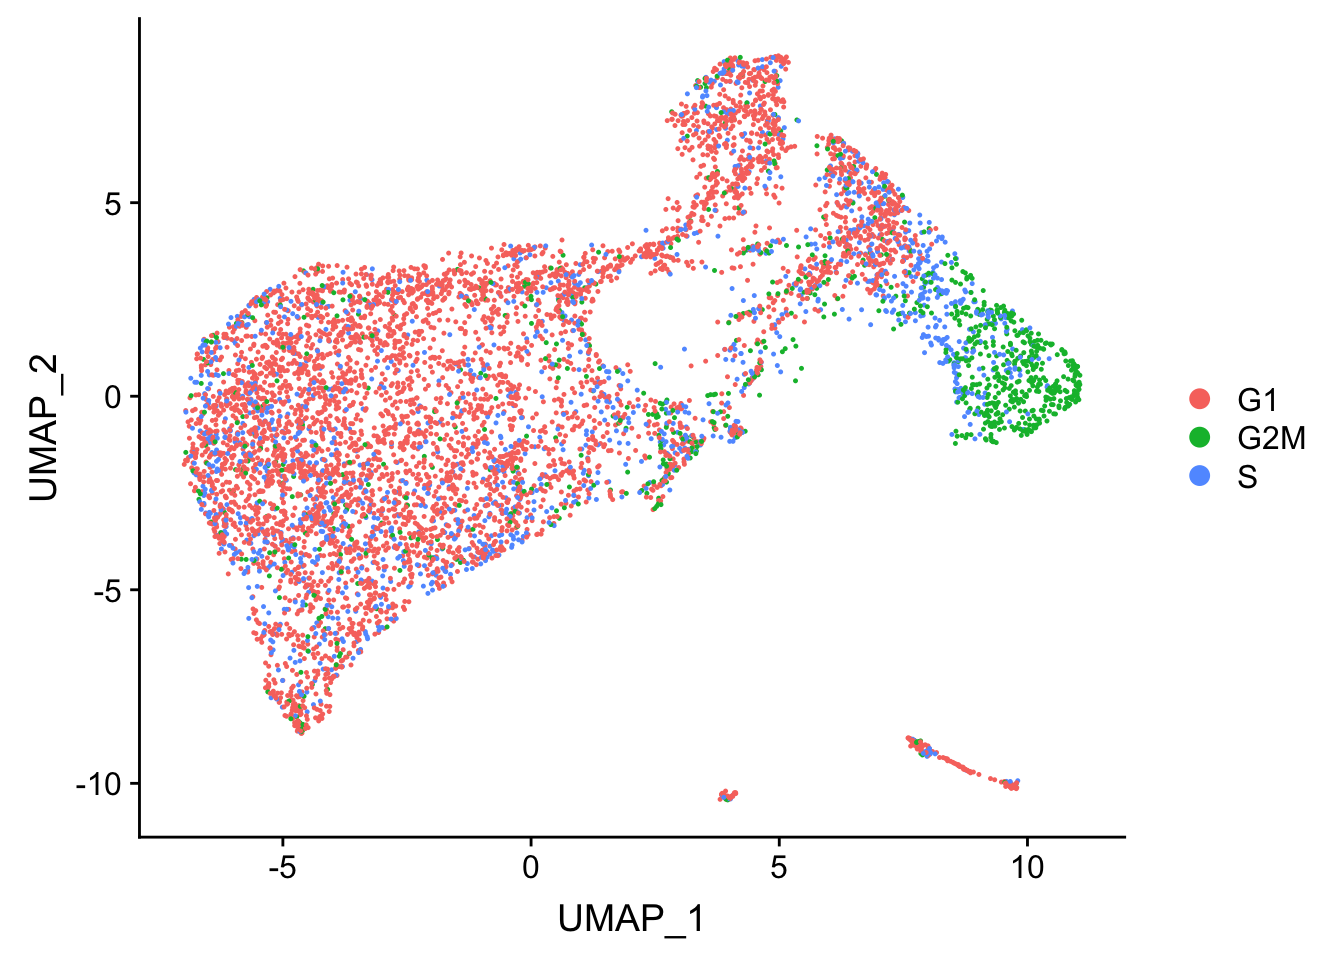
\includegraphics{plots_and_edgeR_analysis_files/figure-latex/unnamed-chunk-14-1.pdf}

\begin{Shaded}
\begin{Highlighting}[]
\NormalTok{fit <-}\StringTok{ }\KeywordTok{glmFit}\NormalTok{(y_for_DE, }\DataTypeTok{design=}\NormalTok{design_matrix2, }\DataTypeTok{dispersion=}\NormalTok{y_for_DE}\OperatorTok{$}\NormalTok{trended.dispersion)}
\end{Highlighting}
\end{Shaded}

Run differential expression

\begin{Shaded}
\begin{Highlighting}[]
\NormalTok{lrt_T <-}\StringTok{ }\KeywordTok{glmLRT}\NormalTok{(fit,}\DataTypeTok{coef =} \StringTok{"ConditionT"}\NormalTok{)}
\KeywordTok{topTags}\NormalTok{(lrt_T)}
\end{Highlighting}
\end{Shaded}

\begin{verbatim}
## Coefficient:  ConditionT 
##           logFC   logCPM       LR       PValue          FDR
## 20567 -2.021209 5.776544 36.92594 1.227027e-09 2.603507e-05
## 20568 -1.947754 5.821635 34.76064 3.728359e-09 3.955416e-05
## 4272  -2.017111 3.155548 25.53381 4.346986e-07 3.074478e-03
## 5407   1.564548 7.921965 24.07899 9.246363e-07 4.904733e-03
## 932   -1.542140 6.925700 23.15304 1.496066e-06 6.348704e-03
## 7981   1.485895 8.495696 21.83559 2.970385e-06 9.235672e-03
## 10765 -1.824441 4.778843 21.78678 3.046927e-06 9.235672e-03
## 21050 -1.614255 4.480648 21.29577 3.936000e-06 1.043926e-02
## 218   -2.123615 3.703030 18.94732 1.343780e-05 3.168035e-02
## 4099  -1.484941 4.503708 18.61541 1.599223e-05 3.393232e-02
\end{verbatim}

\begin{Shaded}
\begin{Highlighting}[]
\KeywordTok{smoothScatter}\NormalTok{(}\DataTypeTok{x=}\NormalTok{lrt_T}\OperatorTok{$}\NormalTok{table}\OperatorTok{$}\NormalTok{logFC, }\DataTypeTok{y=}\OperatorTok{-}\KeywordTok{log10}\NormalTok{(lrt_T}\OperatorTok{$}\NormalTok{table}\OperatorTok{$}\NormalTok{PValue))}
\end{Highlighting}
\end{Shaded}

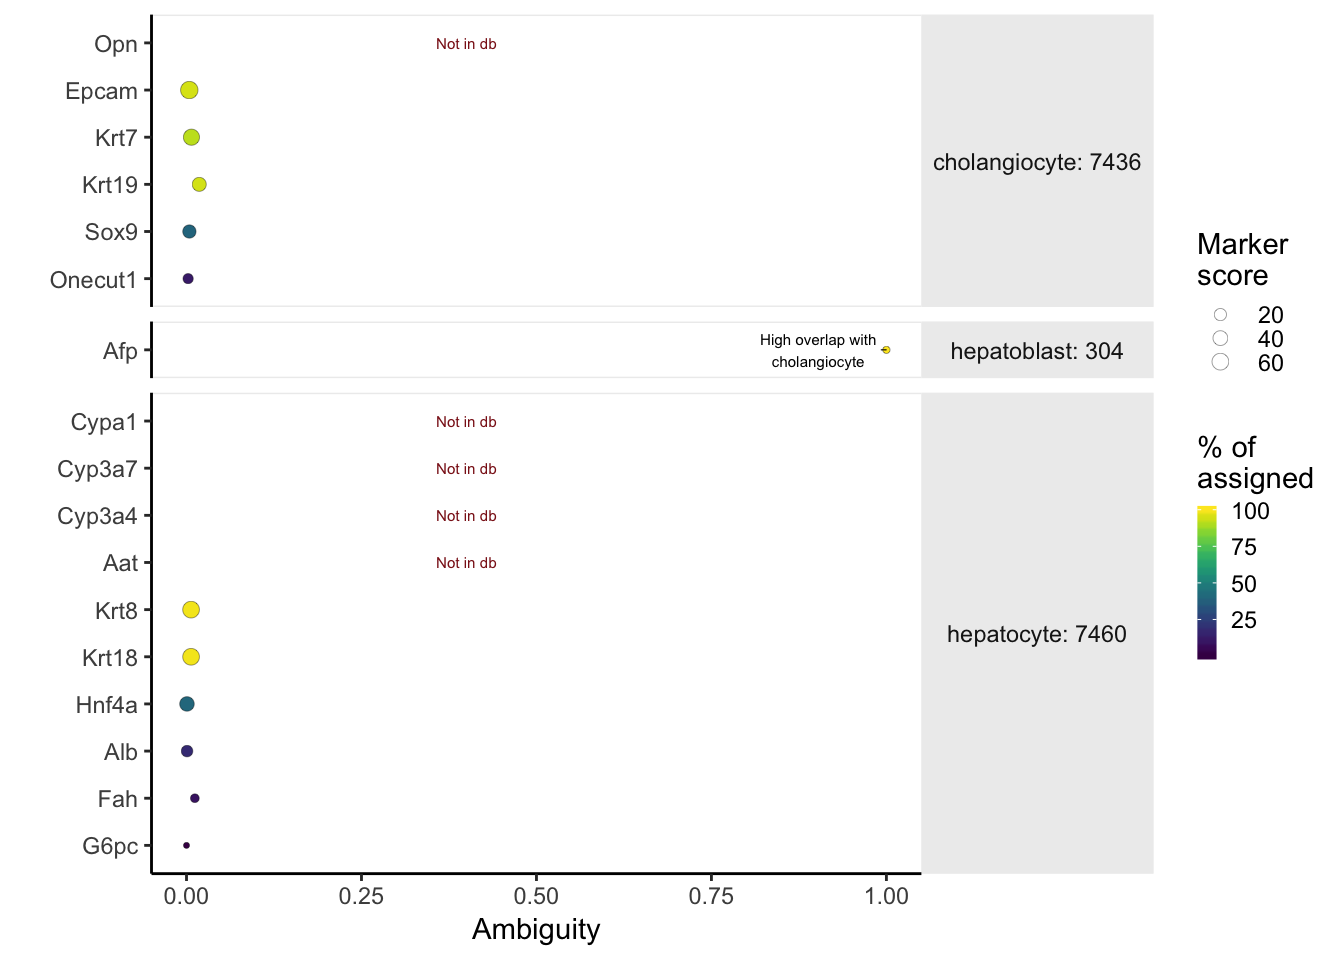
\includegraphics{plots_and_edgeR_analysis_files/figure-latex/unnamed-chunk-15-1.pdf}

\begin{Shaded}
\begin{Highlighting}[]
\NormalTok{lrt_Y <-}\StringTok{ }\KeywordTok{glmLRT}\NormalTok{(fit,}\DataTypeTok{coef =} \StringTok{"ConditionY"}\NormalTok{)}
\KeywordTok{topTags}\NormalTok{(lrt_Y)}
\end{Highlighting}
\end{Shaded}

\begin{verbatim}
## Coefficient:  ConditionY 
##           logFC   logCPM       LR       PValue          FDR
## 7884   3.111090 5.124186 63.11040 1.954390e-15 4.146825e-11
## 19778 -6.925106 4.261791 60.14461 8.813784e-15 6.277676e-11
## 10605  5.996092 4.401853 60.13077 8.875967e-15 6.277676e-11
## 2146  -6.101469 4.897238 56.16611 6.659975e-14 3.532784e-10
## 19779 -5.406648 5.926350 55.61946 8.794857e-14 3.732186e-10
## 9896   2.575217 5.302143 49.54432 1.939401e-12 6.858368e-09
## 10604  4.171126 6.787090 43.93066 3.402174e-11 1.031248e-07
## 10606  5.445078 3.702405 39.88590 2.692400e-10 7.140918e-07
## 6841   4.895458 3.969102 39.58812 3.135855e-10 7.392953e-07
## 10607  5.024080 4.055661 38.14559 6.565799e-10 1.393131e-06
\end{verbatim}

\begin{Shaded}
\begin{Highlighting}[]
\KeywordTok{smoothScatter}\NormalTok{(}\DataTypeTok{x=}\NormalTok{lrt_Y}\OperatorTok{$}\NormalTok{table}\OperatorTok{$}\NormalTok{logFC, }\DataTypeTok{y=}\OperatorTok{-}\KeywordTok{log10}\NormalTok{(lrt_Y}\OperatorTok{$}\NormalTok{table}\OperatorTok{$}\NormalTok{PValue))}
\end{Highlighting}
\end{Shaded}

\includegraphics{plots_and_edgeR_analysis_files/figure-latex/unnamed-chunk-15-2.pdf}

\begin{Shaded}
\begin{Highlighting}[]
\NormalTok{lrt_YT <-}\StringTok{ }\KeywordTok{glmLRT}\NormalTok{(fit,}\DataTypeTok{coef =} \StringTok{"ConditionYT"}\NormalTok{)}
\KeywordTok{topTags}\NormalTok{(lrt_YT)}
\end{Highlighting}
\end{Shaded}

\begin{verbatim}
## Coefficient:  ConditionYT 
##          logFC   logCPM        LR       PValue          FDR
## 8189  4.254222 5.266445 102.16111 5.118504e-24 1.086044e-19
## 18607 3.677992 7.524964  97.26333 6.069397e-23 6.439023e-19
## 3301  4.632456 3.424569  89.25656 3.467905e-21 2.452733e-17
## 17419 3.812053 6.860603  85.49128 2.327259e-20 1.115711e-16
## 5615  3.239965 6.502345  85.17509 2.730811e-20 1.115711e-16
## 7884  3.605549 5.124186  84.88959 3.154995e-20 1.115711e-16
## 910   6.426154 2.307243  82.11934 1.281128e-19 3.883281e-16
## 10372 3.805925 7.716616  81.02243 2.231706e-19 5.919042e-16
## 17420 3.635031 6.225942  76.85862 1.836451e-18 4.329536e-15
## 21134 3.736414 5.636069  74.42870 6.286836e-18 1.333941e-14
\end{verbatim}

\begin{Shaded}
\begin{Highlighting}[]
\KeywordTok{smoothScatter}\NormalTok{(}\DataTypeTok{x=}\NormalTok{lrt_YT}\OperatorTok{$}\NormalTok{table}\OperatorTok{$}\NormalTok{logFC, }\DataTypeTok{y=}\OperatorTok{-}\KeywordTok{log10}\NormalTok{(lrt_YT}\OperatorTok{$}\NormalTok{table}\OperatorTok{$}\NormalTok{PValue))}
\end{Highlighting}
\end{Shaded}

\includegraphics{plots_and_edgeR_analysis_files/figure-latex/unnamed-chunk-15-3.pdf}
TODO

\begin{Shaded}
\begin{Highlighting}[]
\CommentTok{#concatenate fastq files }
\CommentTok{# general gene names}
\CommentTok{#scatter plot of replicates}
\end{Highlighting}
\end{Shaded}


\end{document}
